\subsection*{Ejercicios MRU:}

\begin{enumerate}

\item Una persona corre a una velocidad constante de 10 km/h. ¿Cuánto tarda en alejarse 5 km? %Rta: 0,5 h.

\item Un nene corre a una velocidad constante de 8 km/h. ¿Cuánto tarda en alejarse 400 m? Expresar la respuesta en horas y en minutos. %Rta: 0,05 h, 3 min.

\item Un auto se mueve a una velocidad constante de 50 km/h. Sale desde el kilómetro 20 de una ruta. ¿Cuánto tarda en llegar al kilómetro 120 de esa ruta? ¿Qué distancia recorrió? %Rta: 2 horas.

\item Una chica empieza a andar en patineta a 15 km/h. Está a 1 kilómetro de un poste (alejándose del poste) ¿Qué tan lejos del poste va a estar luego de 2 horas?

\item Una chica está por escalar una palestra. La altura de la palestra es de 20 metros. Si sube con una velocidad de 2 metros por segundo (m/s), ¿cuánto tarda en escalarla?

\item Un ciclista se mueve a 20 km/h. Luego de 5 horas se cansa, y se empieza a mover a 15 km/h. ¿Qué distancia recorre hasta cansarse? ¿Qué distancia recorre en 2 horas? ¿Qué distancia recorre en 8 horas? ¿Cuánto tarda en recorrer 160 km? %Rta: 100 km, 40 km, 145 km, 9 horas.

\item Una auto parte del kilómetro 80 de una ruta a una velocidad constante de 100 km/h. Otro auto parte del kilómetro 20 de la misma ruta a una velocidad de 120 km/h. ¿En qué kilómetro se encuentran? ¿Cuánto tiempo pasa desde que salen hasta que se encuentran? %3 hs, 380km

\item Está Jerry huyendo a 2m/s constantes de Tom, quien está 20m detrás suyo. Tom lo persigue a 3m/s constantes. Cuánto tarda Tom en alcanzarlo? A qué distancia de su posición inicial lo alcanza?

\item Un tren sale de una estación a 60km/h yendo hacia el este. Otro tren sale de otra estación (700 km al este de la original) 90 minutos más tarde, a 80km/h yendo hacia el oeste. Calcular cuánto tardan en chocar y a qué distancia de las estaciones.

\end{enumerate}

\hrule

\subsection*{Ejercicios MRUV:}

\begin{enumerate}
    \item Un auto inicialmente quieto empieza a acelerar, siendo su aceleración constante 10 m/s$^2$. ¿Cuánto tiempo pasa hasta que se alejó 2000 m de su posición inicial? ¿En cuánto tiempo recorre los primeros 1000 m? ¿Cuánto tiempo tarda hasta llegar a una velocidad de 30 m/s? ¿Qué distancia recorre hasta llegar a una velocidad de 40 m/s?
    
    \item Un auto va a 45 m/s por una calle. El conductor ve un nene a 500m en medio de la calle y clava los frenos. La desaceleración es -100 m/s$^2$. ¿Cuánto tarda en detenerse? ¿Cuánta distancia recorre hasta detenerse? ¿Atropella al nene? 
    
    \item Un auto va a 135 m/s por una ruta. Al llegar al kilómetro 10 de dicha ruta empieza a acelerar de manera constante a 20 m/s$^2$ hasta llegar al kilómetro 20 de la ruta. ¿Cuál es la velocidad en el kilómetro 15 de la ruta y cuánto tarda en llegar a este? ¿Y para el kilómetro 20? 
    
    \item La velocidad de un auto a las 15:00 es 100 km/h. La velocidad del mismo auto a las 16:00 es 120 km/h. Suponiendo que aceleró de manera uniforme, ¿cuánto vale la aceleración? Expresar la respuesta en km/h$^2$ y en m/s$^2$.

    \item La velocidad de un auto en el kilómetro 60 de la ruta es 100 km/h. La velocidad del mismo auto en el kilómetro 70 es 120 km/h. Suponiendo que aceleró de manera uniforme, ¿cuánto vale la aceleración? Expresar la respuesta en km/h$^2$ y en m/s$^2$. %Rta: 220 km/h$^2$; 0,0170 m/s$^2$.

    \item Un chico tira una piedra para arriba desde un edificio. La velocidad inicial de la piedra es 30 m/s. El edificio tiene 20 metros de alto. ¿Cuánto tarda en volver a la altura inicial? ¿Y en llegar al suelo? La aceleración de la gravedad es -10m/s$^2$. %Rta: 6 s; 6,60 s
    
    \item Un ciclista en una carrera va a 72 m/s. Al llegar a una bajada acelera a 5 m/s. La bajada tiene 360 metros de largo. Luego, siguiendo con el envión de la bajada, recorre medio kilómetro de camino llano. Al terminar el camino llano llega a una subida de 180 metros en la cual desacelera a 6 m/s. Luego de la subida sigue sin acelerar por 1 kilómetro y llega a la meta. ¿Cuánto tarda en llegar a la meta? ¿A qué velocidad llega?

    \item Un avión parte desde los 50m a una velocidad de 7m/s con una aceleración constante y carretea 1800 m por la pista durante 30 segundos hasta despegar.

    \begin{enumerate}
    \item Calcular la aceleración. % 3,533 m/s^2
    \item Obtener la ecuación horario de la velocidad del avión.
    \item Calcular la velocidad con la que despega. % 113 m/s
    \item ¿Cuánto tarda en recorrer el primer kilómetro? % 21,9 s
    \item ¿Qué distancia recorre en los últimos 10s?
    \end{enumerate}

    \item Un cocinero persigue a una rata. La rata está 10 m delante, huyendo con una velocidad constante de 8 km/h. El cocinero, inicialmente yendo a 10km/h, tiene una aceleración de $1,5$ m/s$^2$.
    \begin{enumerate}
        \item Calcular cuánto tarda en alcanzar a la cucaracha.
        \item Calcular cuándo la alcanza.
        \item Calcular la velocidad del cocinero al alcanzarla.
    \end{enumerate}

    \item Un ratón pasa frente a un gato a 7,2 km/h. Medio segundo más tarde, el gato reacciona y empieza a acelerar a 2m/s$^2$ hasta alcanzar al gato. Calcular cuánto tarda en alcanzarlo y dónde.


    \item Un auto parte hacia el este desde el km 10 de una ruta, con una velocidad inicial de $18 km/h$ y una aceleración de $1,296 km/h^2$. Una hora y media más tarde, otro auto 400km al este parte hacia el oeste desde el reposo con una aceleración de $0,002 m/s^2$. Calcular cuánto tardan en contrarse
\end{enumerate}


\newpage
\subsection*{Tiro Vertical y caída libre}

\begin{enumerate}
\item Se arroja hacia arriba una pelota con una velocidad inicial de 100 m/s. 
\begin{enumerate}
    \item ¿A qué altura y velocidad se encuentra luego de 5 segundos?

    \item ¿Cuánto tarda en llegar al suelo?  ¿A qué velocidad toca el suelo?
\end{enumerate}

\item Se arroja hacia arriba una moneda desde una altura de 30 m con una velocidad inicial de 150 m/s. 
\begin{enumerate}
    \item ¿A qué altura y velocidad se encuentra luego de 5 segundos?

    \item ¿Cuánto tarda en llegar al suelo?  ¿A qué velocidad toca el suelo? %Rta: 30,8s; -151,84 m/s

    \item ¿En qué momentos está a una altura de 10 m? %Rta: -0,13s y 30,74s
\end{enumerate}

\item Se dispara hacia arriba un cañón cuya bala sale a 1500 m/s desde una altura de 100 m. 
\begin{enumerate}
    \item ¿Cuánto tarda en llegar al suelo?  ¿A qué velocidad toca el suelo? %Rta: 306 s y -1500 m/s

    \item ¿Cuál es la altura máxima que alcanza?
\end{enumerate}

\item Una persona dispara un arma desde la calle hacia arriba. 100 metros arriba de la persona hay una bandera. Decir en qué momentos la bala se encuentra a 15 metros de la bandera y a qué velocidad está yendo.

\item Una persona deja caer un globo lleno de agua desde una altura de 60 m. Desde
el suelo, una persona arroja hacia arriba
un dardo apuntado hacia el globo. El dardo tiene una velocidad inicial de 35 m/s.
\begin{enumerate}
    \item Calcular cuánto tiempo pasa hasta que el
    globo es pinchado.
    \item Calcular la altura a la que el globo se pincha.
    \item Calcular las velocidades justo antes de la colisión.
\end{enumerate}

\item Un técnico está subiendo por las escaleras de una torre de comunicaciones que tiene 130 metros de altura. En la cima de la torre su compañero está por comer un caramelo pero se le cae
\begin{enumerate}
    \item Calcular cuánto tiempo pasa hasta que el
    globo es pinchado.
    \item Calcular la altura a la que el globo se pincha.
    \item Calcular las velocidades justo antes de la colisión.
\end{enumerate}

\item Una nena tira una piedra hacia arriba, un segundo más tarde otra. Sabiendo que las velocidades iniciales de las piedras son 20 km/h, calcular cuánto tardan en estar a la misma altura y esa altura.
\end{enumerate}

\subsection*{Ejercicios Dinámica}

\begin{enumerate}
\item A un cuerpo se le aplica una fuerza de 400 N y tiene una masa de 24 kg, ¿cuánto vale su aceleración?
%Rta: 16,7 m/s^2

\item A un cuerpo se le aplica una fuerza de 45.000 N y tiene una masa de 15 toneladas, ¿cuánto vale su aceleración?
%Rta: 3 m/s^2

\item A un cuerpo se le aplica una fuerza de 50 N y tiene una masa de 40 g, ¿cuánto vale su aceleración?
%Rta: 1250 m/s^2

\item Un cuerpo se encuentra bajo el efecto de una fuerza de 1650 N. Su aceleración es 13,25 m/s$2$, ¿cuánto vale su masa? Expresar el resultado en kg y en g. %Rta: 124 kg y 124.000 g

\item Un cuerpo se encuentra bajo el efecto de una fuerza de 1.000.000 N. Su aceleración es 2 m/s$^2$, ¿cuánto vale su masa? Expresar el resultado en kg, en g y en toneladas. %Rta: 500.000 kg; 500.000.000 g; 500 toneladas

\item Un cuerpo tiene una masa de 25 kg y está acelerando a 14 m/s$^2$, ¿cuánto vale la fuerza total ejercida al cuerpo? Expresar el resultado en N y en kgf. %Rta: 350N y 35,7 kgf.


\item Una persona tiene una masa de 60 kg y está en la superficie terrestre, ¿cuánto vale la fuerza total ejercida al cuerpo? Expresar el resultado en N y en kgf. %Rta: 588 y 60 kgf.

\end{enumerate}


\newpage
\subsection*{Ejercicios unidades}

\begin{enumerate}
\item Calcular cuántos kilogramos son  300 gramos de manzanas.

\item Calcular cuántas horas, minutos y segundos son 24.320 segundos.

\item Calcular cuántos mg son 7 kg de peras.

\item Calcular el largo en dm de una ruta de 4000 km de largo.

\item Calcular el volumen en mL de una pileta de 80L.

\item Calcular el volumen en dm$^3$ de una botella de 2 litros.

\item 9m$^2$ a cm$^2$

\item 8cm$^2$ a mm$^2$

\item 50mm$^2$ a dm$^2$

\item 2km$^2$ a cm$^2$

\item 8m$^3$ a cm$^3$

\item 15cm$^3$ a mm$^3$

\item 30mm$^3$ a dm$^3$

\item Se tiene un campo de 4 km$^2$. Expresarlo en millas$^2$.

\item $162 \dfrac{\text{km}}{\text{h}}$ a $\dfrac{\text{m}}{\text{s}}$.

\item $126 \dfrac{\text{m}}{\text{s}}$ a $\dfrac{\text{km}}{\text{h}}$.


\item Pasar a $\dfrac{kg \cdot m^2}{s\cdot h^2}$:
$$
\dfrac{\text{libra}^2 \cdot pie \cdot milla}{kg \cdot dia^3}
$$
\end{enumerate}


\subsection*{Ejercicios MCU y MCUV}
\begin{enumerate}[label=\arabic*)]

\item Un ventilador de 32cm de radio se enciende y empieza a girar con una aceleración de $\alpha = 0,7 \dfrac{\text{rad}}{s^2}$. Calcular su $\omega$ y sus vueltas dadas luego de 4 s.

\item Hay dos partículas girando alrededor de un punto con mismo radio. La primera partícula describe un MCU con $f = 30$ RMP. La segunda partícula comienza 20º detrás de la primera, describiendo un MCU con $f_0 = 1$ RPM y $\alpha =2\pi$ rad/s$^2$. Calcular cuánto tardan en encontrarse.

\item Hay dos partículas, ambas describiendo MCUVs. Datos de la primera: $\omega_{0-1}=10\pi$ rad/s, $\alpha_1=1\pi$ rad/s. Datos de la segunda: $\omega_{0-2}=12\pi$ rad/s, $\alpha_2=2\pi$ rad/s. Sabiendo que la segunda está $1,5\pi$ delante de la primera. Cuánto tardan en encontrarse? Cuántas vueltas hace cada una hasta el encuentro?

\item Hay dos partículas girando en el mismo sentido alrededor de un punto, con $R=5$m. La primera hace un MCU y la segunda un MCUV. Datos de la primera partícula: $v_t=72$ m/s. Datos de la segunda partícula: $\omega_0=25$ rad/s, $\alpha= 2$ rad/s$^2$. Calcular cuánto tardan en encontrarse.

\item Una partícula parte desde el reposo empezando a girar alrededor de un círculo en sentido horario describiendo un MCUV con $\alpha = 4\pi$ rad/s$^2$. Desde el lado opuesto otra partícula gira en sentido antihorario con $\alpha = 6\pi$ rad/s$^2$ y $\omega_0=2\pi$ rad/s. Teniendo en cuenta que ambas comienzan desde el mismo punto, calcular cuánto tardan en volver a encontrarse y dónde lo hacen.

\item Una partícula comienza a girar en sentido horario a $\omega=1,5\pi$ rad/s. Otra partícula comienza a girar en el mismo sentido 20º detrás del punto inicial de la anterior 500 ms después. $f_2 = 0,75$ Hz y empieza a desacelerar con $\alpha_2 = 0,2\pi$ rad/s$^2$. Calcular cuánto tiempo pasa hasta que se encuentran y dónde.

\item Calcular cuánto tardan en chocar dos vehículos que giran en sentidos opuestos alrededor de la misma pista de 4km de diámetro, que arrancan del reposo y tienen una aceleración tangencial de $1500 \dfrac{km}{h^2}$. Obtener la aceleración total de cada uno 10 segundos antes que choquen.

\item La velocidad tangencial de un diente del engrajane 1 es de 7 m/s. Averiguar $v_{t2}$ y $\omega_2$.

\begin{figure}[H]
    \centering
    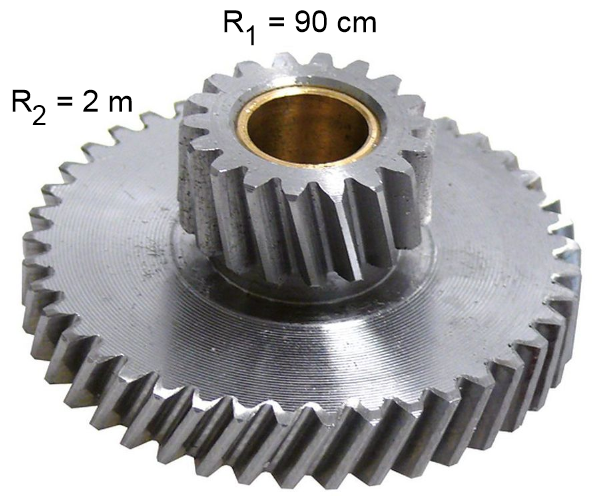
\includegraphics[width=0.3\linewidth]{images/engranaje_1.png}
\end{figure}

\item La velocidad angular $\omega_1 = 3,3\dfrac{\text{rad}}{s}$. Averiguar $v_{t\,2}$ y $\omega_2$.

\begin{figure}[H]
    \centering
    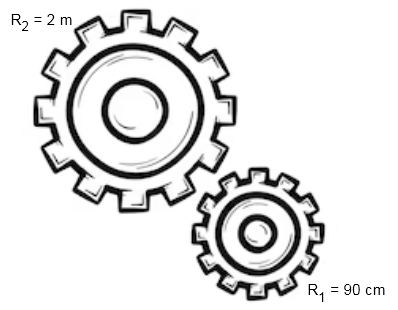
\includegraphics[width=0.4\linewidth]{images/engranaje_2.png}
\end{figure}    
\end{enumerate}
